%-------------------------------------------------------------------------------------------
% Vorlage erstellt von sli92
% Latex für Einsteiger: http://latex.mschroeder.net/#textformatierung
% Formeln in Latex: http://www.hosi.de/latex/mathe.htm
%-------------------------------------------------------------------------------------------
%PRÄAMBEL
%-------------------------------------------------------------------------------------------

\documentclass[a4paper,14pt,headsepline]{scrartcl}

\usepackage[ngerman]{babel}
\usepackage[utf8]{inputenc}
\usepackage{fancyheadings}
\usepackage{graphicx}
\usepackage{eurosym}

% Absatzeinrückung
%++++++++++++++++++++++++++
%\setlength{\parskip}{5pt}
%\setlength{\parindent}{0pt}

\setlength{\parskip}{1.5em}
\setlength{\parindent}{0pt}

% Kopf- und Fußzeile
%++++++++++++++++++++++++++

\pagestyle{fancy}
\lhead{\bfseries netcon}
%\chead{Lipp}
\rhead{\nouppercase{\leftmark}}

%C für Center
\fancyfoot[C]{ \thepage}

%-------------------------------------------------------------------------------------------
%DOKUMENT
%-------------------------------------------------------------------------------------------

\begin{document}

% Titelseite
%++++++++++++++++++++++++++
\author{Lipp, Pietryka} 
\title{Diplomarbeit: netcon} 
\date{} 
\maketitle

\newpage

\section*{Zusammenfassung}
\newpage

\section*{Abstract}
\newpage

\section*{Danksagung}
\newpage

\section*{Einleitung}
In vielen Fällen ist bereits eine Infrastruktur vorhanden, sei es ein Firmen- oder. Heimnetzwerk auf Ethernet-Basis. Wieso sollte man dieses nicht nutzen, um einfache Steuer- und Messaufgaben zu realisieren? Wieso müssen für einfachste Anwendungen, wie z.B. die Überwachung von Wettergrößen, bereits neue Messsysteme angeschafft werden? Das dafür notwendige Netzwerk, ist häufig bereits vorhanden. Vor allem Privatanwender wünschen sich oft eine kostengünstige Möglichkeit. Netcon hat das Ziel, diesem Bedürfnis nachzukommen und eine einfache Lösung anzubieten. Zudem stehen alle erstellten Entwicklungen unter der OpenSource-Lizenz. 

Diese Diplomarbeit soll im ersten Teil einen Überblick verschaffen, wie so ein netcon-System in den Grundzügen aufgebaut ist. Danach geht es zum Grundlagen-Kurs, der je nach Bedarf gelesen werden kann um dann die zwei großen Kapitel Hardware und Software zu verstehen.

Viel Spaß!

\newpage

% Inhaltsverzeichnis
%++++++++++++++++++++++++++
\tableofcontents
\newpage

%Inhalt
%++++++++++++++++++++++++++

\section{Überblick}

\subsection{Was ist netcon?}
\textbf{Netcon} bezeichnet ein flexibles Mess- und Steuersystem zur Einbindung in ein bestehendes Ethernet-Netzwerk. 

Das System garantiert kein Echtzeitverhalten, weshalb es auch nur für nicht zeitkritische Anwendungen geeignet ist. Grund hierfür ist die Wahl der Kommunikationsschnittstelle, die mit dem Internet Protocol (IP) über Ethernet, zeitkritische Übertragungen nicht sicherstellt. Die Einbindung in ein bestehendes Firmen- oder Heimnetzwerk ist damit aber umso einfacher. Bis auf die Erstellung von netcon-kompatiblen Modulen ist im einfachsten Fall nur ein handelsüblicher Router erforderlich.

Im Gegensatz zu vielen anderen Systemen ist netcon kein Produktpaket, das so im Geschäftsregal stehen soll, sondern vielmehr eine Vereinbarung bzw. Protokoll, woran sich Aktor- oder Sensormodule halten müssen um gemeinsam in einem System zu funktionieren. Dazu stellt die Diplomarbeit Firmware für einige Mikrocontroller-Systeme und eine plattformunabhängige Verwaltungsumgebung zur Verfügung. 

Im Rahmen dieser Diplomarbeit wurden also netzwerkfähige Steuer- und Messmodule geschaffen, auf die in Kapitel \textbf{Hardware} noch weiter eingegangen wird. Die zentrale Software zur Verwaltung der Module wird in Kapitel \textbf{Software} näher beschrieben. 

Vorher wird der grundlegende Aufbau des netcon-Systems erklärt und benötigte Grundlagen behandelt.

\subsection{Grundlegender Aufbau}
Vorausgesetzt das Netzwerk besteht bereits, sind weiters netzwerkfähige Aktor- und Messmodule, sowie eine Betriebsumgebung für die Verwaltungssoftware notwendig. Diese Umgebung kann jeder Computer sein, der mit einer Java Virtual Runtime und einem httpd-Webserver mit PHP Unterstützung ausgestattet ist. Die Module müssen sich an die Konventionen halten, die in zwei Protokollen spezifiziert sind. Dazu näheres in Kapitel Hardware. Abb. 1 zeigt den grundlegenden Aufbau eines solchen Systems.

Grafik

\newpage

\section{Grundlagen}

\section{Hardware}
\subsection{Auswahl des Ethernet Controllers}
Damit ein Mikrocontroller über das Ethernet kommunizieren kann, wird eine entsprechende Hardware benötigt, der sogenannte Ethernet Controller. Ein Ethernet Controller übernimmt dabei die Aufgaben der OSI-Schichten 1(Physical) und 2(Data-Link). Der Controller benötigt zudem einen entsprechend großen Empfangspuffer, um mindestens einen vollwertigen Ethernet-Frame(1542 Byte) aufzunehmen zu können. Dabei standen für 8-Bit Mikrocontroller vorerst zwei verschiedene Bausteine zur Auswahl, einmal der CP2200 von SiLabs, und einmal der ENC28J60 von Microchip. Beide Controller haben, was die Netzwerkkommunikation angeht, so ziemlich die selben Features, der gravierende Unterschied liegt jedoch in der Ansteuerung dieser. Der CP2200 wurde von SiLabs, wie es scheint, nur für die Verwendung mit einem Mikrocontroller vom Typ 8051 entwickelt, die Ansteuerung erfolgt deshalb über einen parallelen Adress-/Datenbus wodurch man mindestens 16 Leitungen und Pins am Mikrocontroller benötigt. Beim ENC28J60 erfolgt die Kommunikation über den SPI-Bus, daher benötigt man nur vier Leitungen(MOSI, MISO, SCK, CS), dadurch hat auch der Netzwerkcontroller selber nur 28 Pins und ist auch im "bastlerfreundlichen" DIP-Gehäuse zu bekommen. Ein anderer Faktor für die Auswahl des ENC28J60 war das Vorhandensein einer günstigen Entwicklungsplatine, es gibt bei Pollin den AVR-NET-IO Bausatz, dieser kostet nur \EUR{20} und enthält alle für die Netzwerkprogrammierung benötigten Komponenten(ATmega32, ENC28J60, RJ-45 Buchse).

\subsection{ENC28J60 Beschaltung}
Die Aussenbeschaltung benötigt neben einigen Standardbauelementen auch einige 1\% Widerstände und einen 1:1 Übertrager, jedoch gib es RJ-45 Buchsen in denen bereits der Übertrager, sowie die LEDs, eingebaut sind.
\begin{figure}[h]
\begin{center}
\fbox{
	%Rahmengroesse	
	\begin{minipage}{0.7 \paperwidth}
	\begin{center}
	%Bildgroesse
	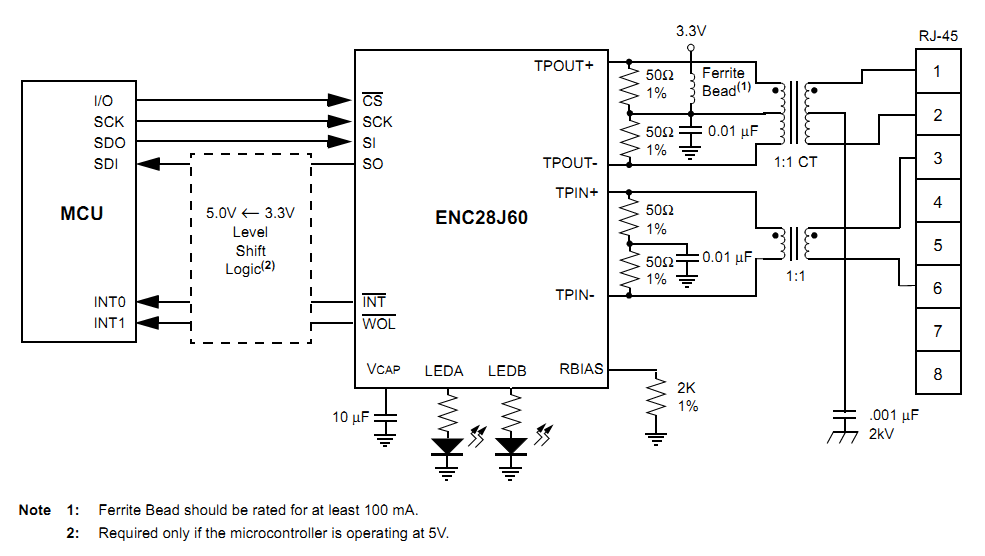
\includegraphics[width=0.7 \paperwidth]{./bilder/enc28j60_beschaltung.png}
	\caption{Aussenbeschaltung ENC28J60}
	\end{center}
	\end{minipage}
}
\end{center}
\end{figure}



\subsection{ENC28J60 Treibersoftware}

\section{Software}

 
\end{document}